\documentclass{article}
\usepackage{tikz}
\usepackage{float}
\usepackage{amsmath}
\usepackage{lmodern}
\usepackage{amssymb}
\usepackage{ifthen}
\usetikzlibrary{calc}
\usetikzlibrary{intersections}
\usetikzlibrary{decorations.markings}
\usetikzlibrary{patterns, patterns.meta}
\usetikzlibrary{shapes}

\begin{document}

\centering

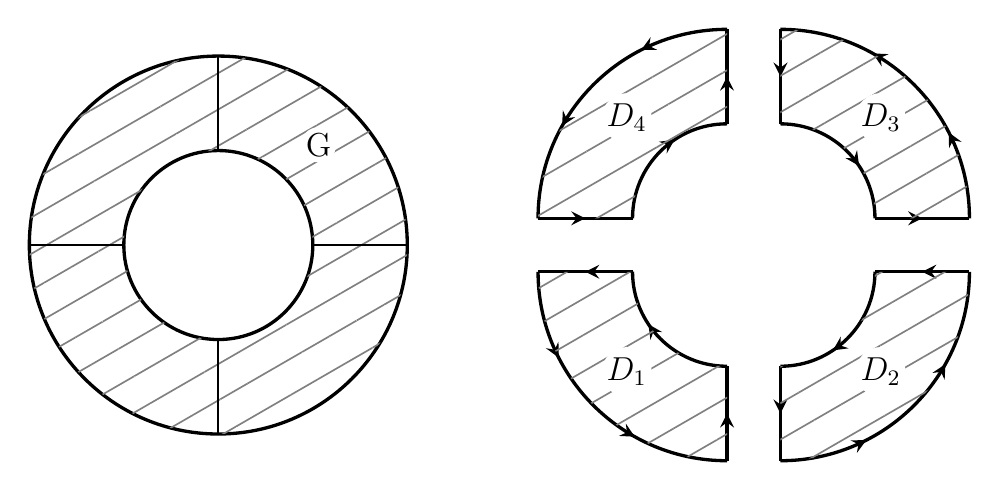
\begin{tikzpicture}[scale=0.8]
\pgfmathsetmacro{\CircleSize}{0.08}     % radius of coordinate circles/dots
% define styles used in this picture
\tikzset{
BigTextFont/.style={font=\large},
every node/.style={font=\normalsize, text=black},
CircleNodeStyle/.style={draw=black, shape=circle, fill=black, minimum size=\CircleSize*2 cm, inner sep=0pt},
arrowstyle/.style={->, >=stealth}}
\pgfmathsetmacro{\PartSplit}{0.6}

% draw  the area
\pgfmathsetmacro{\InnerCircleRadius}{1.5}
\pgfmathsetmacro{\OuterCircleRadius}{3.0}
\draw[very thick] (0,0) circle [radius=\InnerCircleRadius];
\draw[very thick] (0,0) circle [radius=\OuterCircleRadius];

% fill area with pattern (even odd rule for exclusion of inner circle)
\fill[even odd rule, pattern={Lines[angle=30, distance=0.4cm, line width=0.6pt]}, pattern color=gray] circle (\InnerCircleRadius) circle (\OuterCircleRadius);

% partitions
\draw[thick] (0,\InnerCircleRadius) -- (0,\OuterCircleRadius);
\draw[thick] (0,-\InnerCircleRadius) -- (0,-\OuterCircleRadius);
\draw[thick] (\InnerCircleRadius, 0) -- (\OuterCircleRadius, 0);
\draw[thick] (-\InnerCircleRadius, 0) -- (-\OuterCircleRadius, 0);

% G area symbol
\pgfmathsetmacro{\NodeRadius}{(\InnerCircleRadius + \OuterCircleRadius)/2}
\node[draw=white, circle, inner sep=0, fill=white, BigTextFont] at (45 : \NodeRadius) {G};

%\def\labels{{$D_{1}$}, {$D_{2}$}, {$D_{3}$}, {$D_{4}$}}

% for leap for making the 4 different partitions
\foreach \StartAngle/\EndAngle/\label in {0/90/{$D_{3}$}, 90/180/{$D_{4}$}, 180/270/{$D_{1}$}, 270/360/{$D_{2}$}} {

% shift each part in a different direction
\pgfmathsetmacro{\xshift}{\PartSplit*cos((\StartAngle+\EndAngle)/2)}
\pgfmathsetmacro{\yshift}{\PartSplit*sin((\StartAngle+\EndAngle)/2)}
\begin{scope}[xshift=8.5cm, shift={(\xshift, \yshift)}]
    % draw the 4 edges of the part, with arrows counterclockwise
    \draw[postaction={decorate}, decoration={
        markings,
        mark = between positions 0.375 and 1 step 0.75 with {\arrowreversed{stealth}}}]
    [very thick] (\StartAngle :\InnerCircleRadius) arc [start angle=\StartAngle, end angle=\EndAngle, radius=\InnerCircleRadius];
    
    \draw[postaction={decorate}, decoration={
        markings,
        mark = between positions 0.3 and 1 step 0.375 with {\arrow{stealth}}}]
    [very thick] (\StartAngle :\OuterCircleRadius) arc [start angle=\StartAngle, end angle=\EndAngle, radius=\OuterCircleRadius];
    
    \draw[postaction={decorate}, decoration={
        markings,
        mark=at position 0.50 with {\arrow{stealth}}}]
    [very thick] (\StartAngle :\InnerCircleRadius) -- (\StartAngle :\OuterCircleRadius);

    \draw[postaction={decorate}, decoration={
        markings,
        mark=at position 0.50 with  {\arrowreversed{stealth}}}]
    [very thick] (\EndAngle :\InnerCircleRadius) -- (\EndAngle :\OuterCircleRadius);
    % fill the contour
    \fill[pattern={Lines[angle=30, distance=0.4cm, line width=0.6pt]}, pattern color=gray] (\EndAngle :\InnerCircleRadius) arc [start angle=\EndAngle, end angle=\StartAngle, radius=\InnerCircleRadius] -- (\StartAngle :\InnerCircleRadius) -- (\StartAngle :\OuterCircleRadius) -- (\StartAngle :\OuterCircleRadius) arc [start angle=\StartAngle, end angle=\EndAngle, radius=\OuterCircleRadius] -- cycle;

    % place a label
    \pgfmathsetmacro{\NodeRadius}{(\InnerCircleRadius + \OuterCircleRadius)/2}
    \pgfmathsetmacro{\NodeAngle}{(\StartAngle + \EndAngle)/2}
    \node[draw=white, circle, inner sep=0, fill=white, BigTextFont] at (\NodeAngle : \NodeRadius) {\label};

\end{scope}
}

\end{tikzpicture}

\end{document}